% !TeX root = ../main.tex
\section{Probability Foundations}\label{sec:probability}

\subsection{Combinatorics of the deck}

All card probabilities flow from one primitive: the number of ways to choose $k$ unordered cards from $n$ distinct cards,
\begin{equation}\label{eq:binom}
\binom{n}{k} \;=\; \frac{n!}{k!\,(n-k)!},
\end{equation}
because every hand in poker is an unordered subset of the deck, and (before any cards are observed) all subsets are equiprobable. Texas Hold'em uses the $k=2$ and $k=5$ cases at the moment cards are assigned to players, and the $k=7$ case at showdown, where the player's effective hand is the \emph{best five-card subset} of the seven available cards.

The number of distinct starting hands is
\begin{equation}
\binom{52}{2} = \frac{52 \cdot 51}{2} = 1326 .
\end{equation}
Suits are strategically interchangeable, so many holdings are equivalent up to suit isomorphism: there are $13$ pocket pairs, $\binom{13}{2}=78$ suited combinations and $78$ offsuit non-pair combinations, giving $169$ \emph{canonical} starting hands. A specific pair such as $Q\spadesuit Q\heartsuit$ has probability $6/1326$ (six suit pairings), a specific suited hand such as $A\spadesuit K\spadesuit$ has probability $4/1326$, and a specific offsuit hand such as $A\spadesuit K\heartsuit$ has probability $12/1326$. These are the weights one must use when aggregating over the canonical classes.

\subsection{Hand-category frequencies}

Table~\ref{tab:ranks} lists the exact number of five-card and seven-card combinations falling into each ranking category, together with the resulting probabilities. The five-card column is a classical computation; we illustrate with two categories and note that the rest follow the same bookkeeping. For a flush, choose the suit ($4$ ways), then choose $5$ of that suit's $13$ cards, and subtract the $10$ straight flushes:
\begin{equation}
4\,\binom{13}{5} - 40 = 5108 .
\end{equation}
For exactly one pair, choose the paired rank ($13$), the pair's suits $\binom{4}{2}=6$, the three distinct kicker ranks from the remaining $12$ ranks $\binom{12}{3}$, and one suit for each kicker ($4^3$):
\begin{equation}
13\,\binom{4}{2}\,\binom{12}{3}\,4^3 = 1098240 .
\end{equation}

The seven-card column counts the best five-card category of each of the $\binom{52}{7} = 133{,}784{,}560$ combinations. The inversions relative to the five-card distribution are striking and consequential. Among seven cards, one pair becomes the \emph{modal} category (about $43.8\%$), while a no-pair high card collapses to $17.4\%$; a player holding five visible community cards plus two hole cards therefore makes at least a pair most of the time. Conversely, straights, flushes, and full houses all become far more common than their five-card frequencies suggest. Figure~\ref{fig:handranks} visualises the distribution on a logarithmic scale spanning five orders of magnitude.

\begin{table}[!t]
\centering
\small
\renewcommand{\arraystretch}{1.32}
\setlength{\tabcolsep}{9pt}
\caption{Exact hand-category frequencies for five-card and seven-card poker hands. Probabilities are relative to $\binom{52}{5}=2{,}598{,}960$ and $\binom{52}{7}=133{,}784{,}560$ combinations respectively. The seven-card column reflects the \emph{best} five-card hand available within each combination.}
\label{tab:ranks}
\begin{tabular}{lrrrr}
\toprule
& \multicolumn{2}{c}{5 cards} & \multicolumn{2}{c}{7 cards} \\
\cmidrule(lr){2-3}\cmidrule(lr){4-5}
Category & Count & Probability & Count & Probability \\
\midrule
Straight flush & $40$ & $0.00154\%$ & $41{,}584$ & $0.0311\%$ \\
Four of a kind & $624$ & $0.0240\%$ & $224{,}848$ & $0.168\%$ \\
Full house & $3{,}744$ & $0.144\%$ & $3{,}473{,}184$ & $2.60\%$ \\
Flush & $5{,}108$ & $0.197\%$ & $4{,}047{,}644$ & $3.03\%$ \\
Straight & $10{,}200$ & $0.392\%$ & $6{,}180{,}020$ & $4.62\%$ \\
Three of a kind & $54{,}912$ & $2.11\%$ & $6{,}461{,}620$ & $4.83\%$ \\
Two pair & $123{,}552$ & $4.75\%$ & $31{,}433{,}400$ & $23.5\%$ \\
One pair & $1{,}098{,}240$ & $42.3\%$ & $58{,}627{,}800$ & $43.8\%$ \\
High card & $1{,}302{,}540$ & $50.1\%$ & $23{,}294{,}460$ & $17.4\%$ \\
\bottomrule
\end{tabular}
\end{table}

\begin{figure}[htbp]
\centering
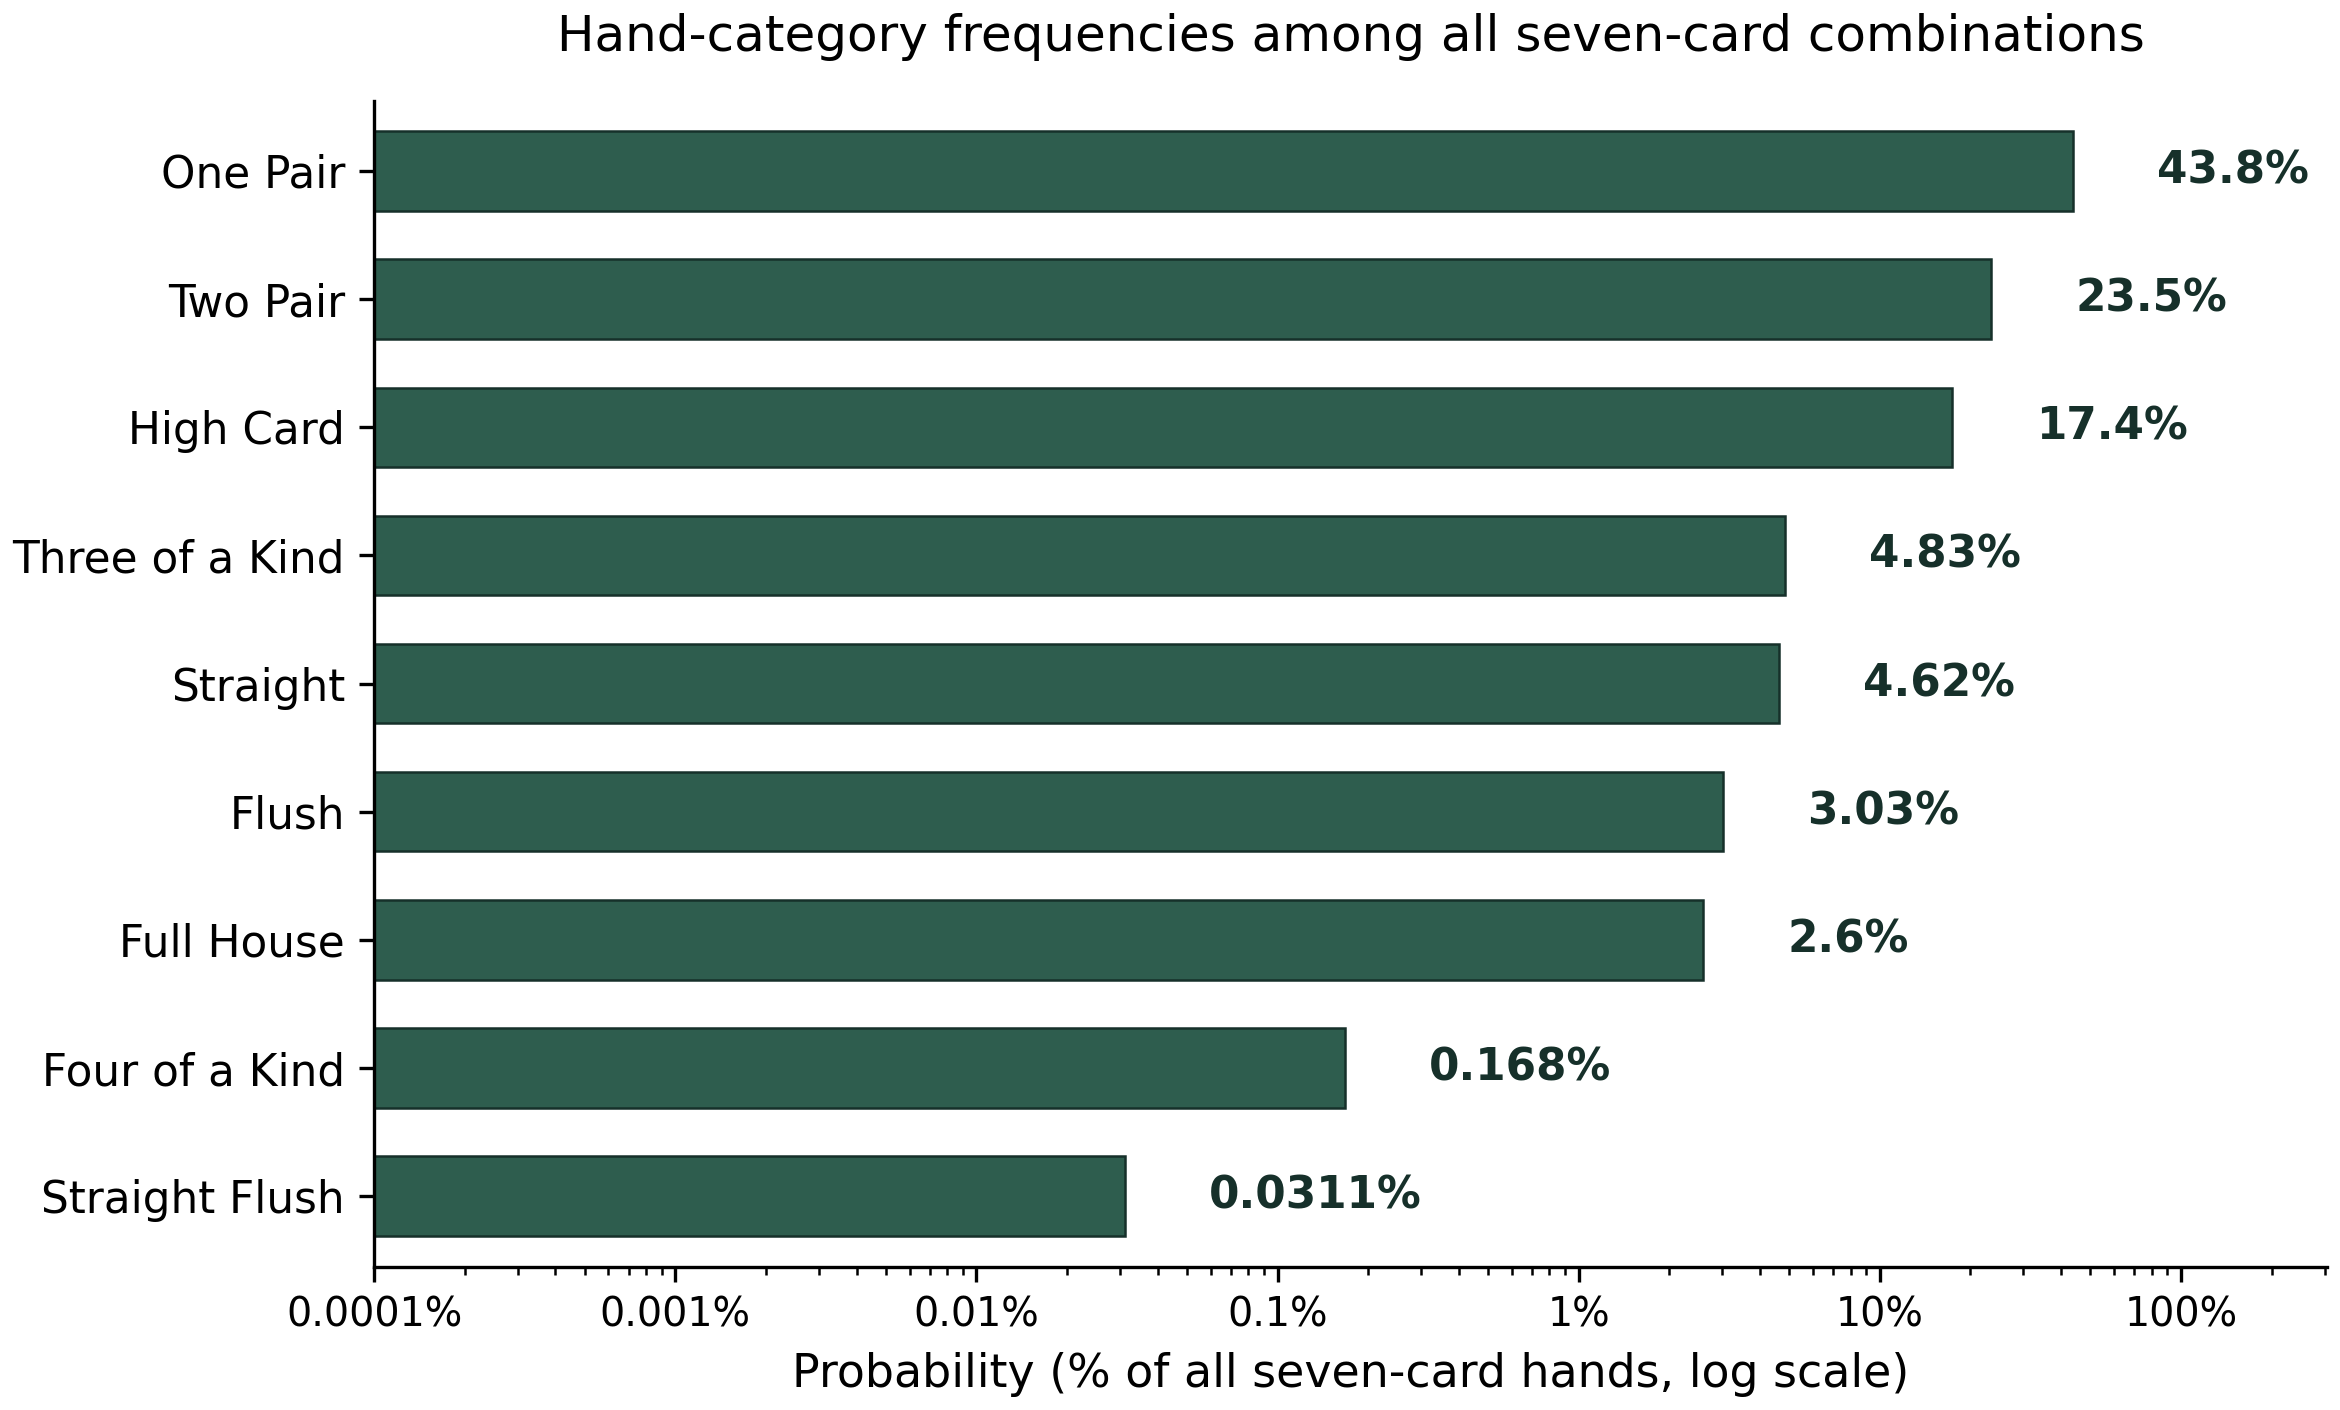
\includegraphics[width=0.92\textwidth]{figures/hand_ranks.png}
\caption{Frequency of each hand category among all $\binom{52}{7}$ seven-card combinations, on a logarithmic probability scale (categories ordered by seven-card frequency). Labels give percentages; the corresponding exact counts appear in Table~\ref{tab:ranks}.}
\label{fig:handranks}
\end{figure}

\subsection{Preflop equity}\label{sec:preflopequity}

The single most useful summary of a starting hand is its \emph{equity}: the probability of winning (with ties counted fractionally) if all remaining cards were dealt and all hands revealed. Equity against a single uniformly random opponent can be computed exactly by enumeration or estimated by simulation; Figure~\ref{fig:preflop} shows the values for all $169$ canonical hands. The structure is instructive. Pocket aces hold about $85\%$ equity; the worst hand, $7\clubsuit 2\diamondsuit$, holds about $35\%$---still far from hopeless heads-up, because even trash occasionally pairs or makes a backdoor straight. Suitedness is worth roughly $2$--$3$ equity points for high-card hands (flush potential), and connectedness adds a fraction of a point (straight potential). The same grid, computed against multiple simultaneous random opponents, compresses dramatically: against five random hands, AA retains roughly $49\%$ equity while $72$o falls under $5\%$, which is why multiway pots systematically reward speculative hands and punish dominated high-card holdings.

\begin{figure}[htbp]
\centering
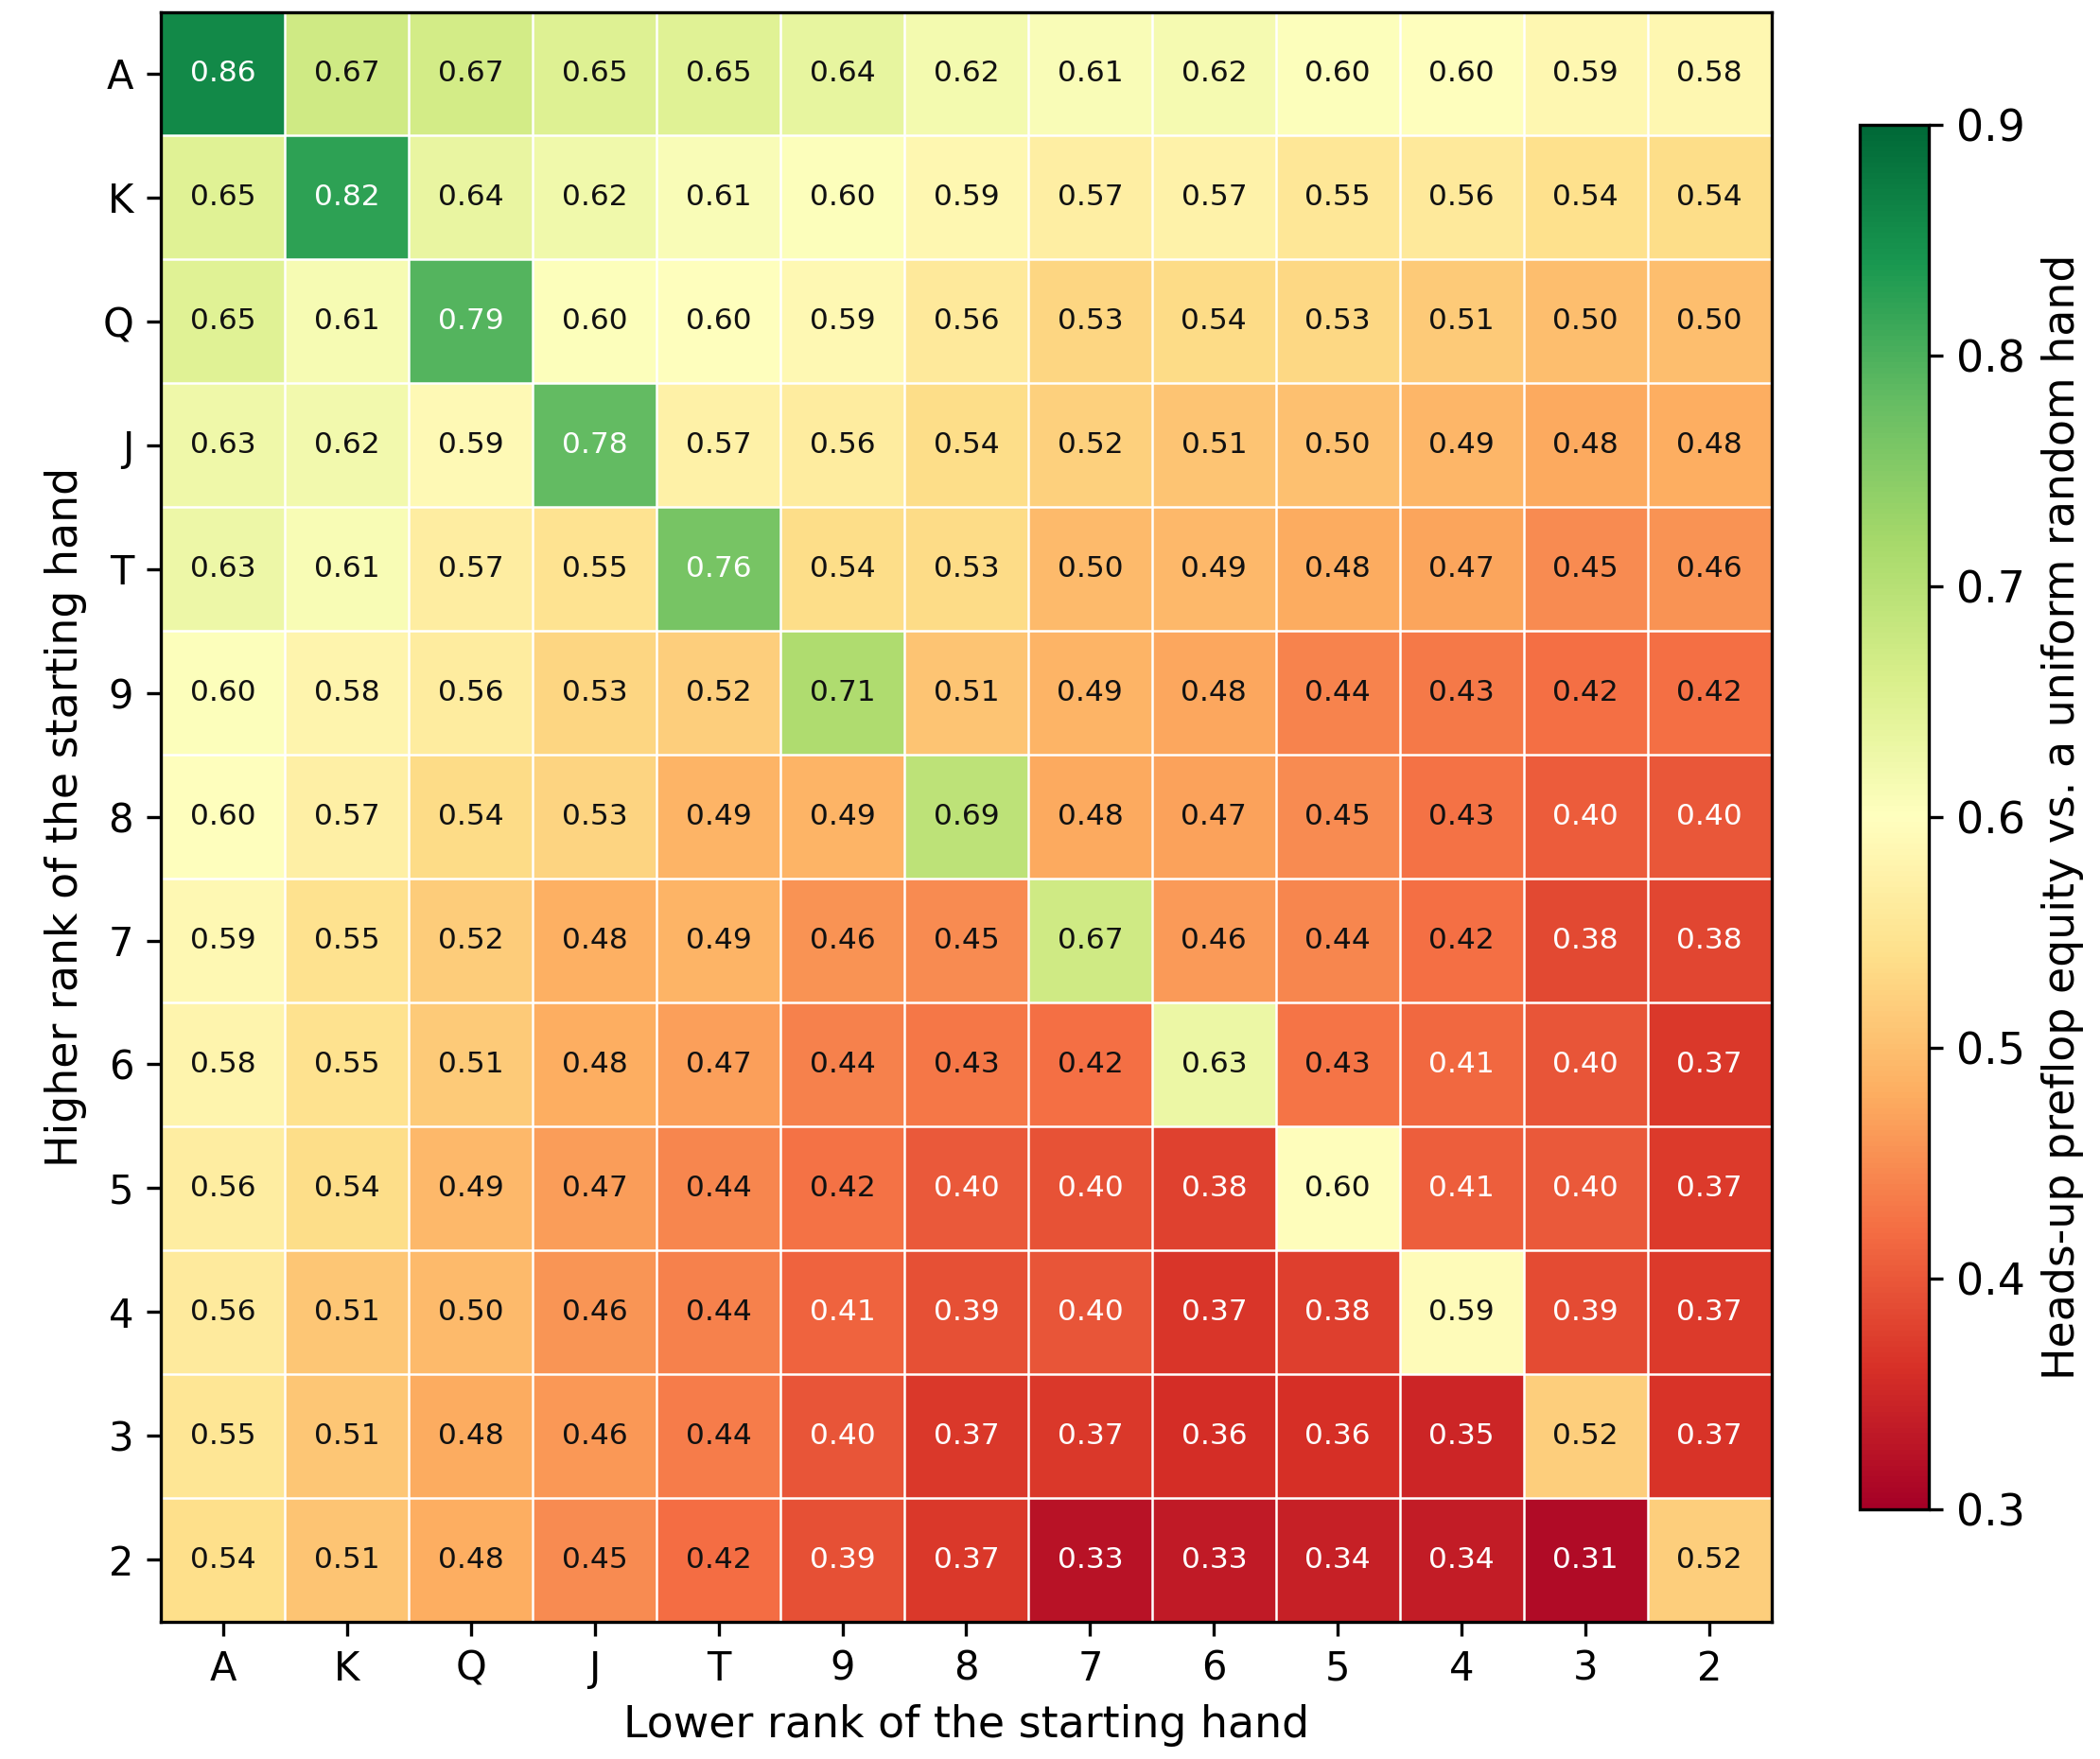
\includegraphics[width=0.86\textwidth]{figures/preflop_equity.png}
\caption{Heads-up preflop equity of all $169$ canonical starting hands against a uniformly random opponent, estimated by Monte Carlo simulation with $4{,}000$ runouts per hand. Values above the diagonal are suited hands; those below are offsuit.}
\label{fig:preflop}
\end{figure}

\subsection{Conditional probability and reads}

Once the flop arrives, hand strength must be conditioned on the visible cards. If a player holds a flush draw---four cards of one suit---then among the $47$ unseen cards, $9$ complete the flush, so by a direct application of the definition of conditional probability,
\begin{equation}\label{eq:flushdraw}
\Pr(\text{flush by river} \mid \text{flop}) = 1 - \frac{\binom{47}{2} - \binom{9}{1}\binom{38}{1} - \binom{9}{2}}{\binom{47}{2}} = 1 - \frac{\binom{38}{2}}{\binom{47}{2}} \approx 0.3497 .
\end{equation}
Poker players memorise the practical rule that follows from \eqref{eq:flushdraw}: with two cards to come, multiply the number of \emph{outs} by $4$; with one card to come, by $2$. The rule is accurate to within a couple of percentage points for the relevant range $1 \le \text{outs} \le 21$ precisely because it is the first-order binomial approximation of \eqref{eq:flushdraw}.

Bayes' theorem is the formal home of \emph{reading} an opponent. Write $H$ for a hypothesis about the opponent's holding (for instance, ``at least one club'') and $E$ for observed evidence (for instance, ``the opponent called a large bet on a two-club board''). Then
\begin{equation}\label{eq:bayes}
\Pr(H \mid E) = \frac{\Pr(E \mid H)\,\Pr(H)}{\Pr(E)},
\qquad
\Pr(E) = \sum_{H'} \Pr(E \mid H')\,\Pr(H') .
\end{equation}
Strong play requires an a priori model $\Pr(H)$ of the opponent's distribution (a \emph{range}) over holdings, and a behavioural likelihood $\Pr(E \mid H)$ describing how the opponent bets with each holding. Expert ``table reading'' is exactly the disciplined application of \eqref{eq:bayes}, updating the range after every action; opponent-modelling systems such as those reviewed by Billings et al.~\cite{billings2002challenge} mechanise the same computation.

\subsection{Pot odds, equity, and expected value}

Suppose the pot currently contains $P$ chips and a player faces a bet of $b$ chips. Calling costs $b$ to contest a pot of $P + b$, so the call is profitable in expectation against the bettor's distribution whenever the caller's equity $\eq$ satisfies
\begin{equation}\label{eq:potodds}
\eq \;>\; \frac{b}{P + b} .
\end{equation}
The right-hand side is called the \emph{pot odds} expressed as a required equity fraction. The inequality follows from a one-line expected-value computation: letting $W$ be the indicator of winning the pot outright (ignoring ties),
\begin{equation}\label{eq:evcall}
\E[\text{profit}] = \eq\,P - (1-\eq)\,b = \eq (P + b) - b ,
\end{equation}
which is positive exactly when \eqref{eq:potodds} holds. As a concrete example: facing a half-pot bet of $b = P/2$, the threshold is $P/2 \div 3P/2 = 1/3$; a player with a nine-out flush draw on the turn ($9/46 \approx 0.196$ from \eqref{eq:flushdraw} with one card to come) does not have direct odds and must either fold or justify the call through \emph{implied odds}---expected additional winnings $I$ on later streets when the draw completes, replacing \eqref{eq:potodds} by
\begin{equation}
\eq \;>\; \frac{b}{P + b + I} .
\end{equation}

Expected value is the fundamental quantity of the entire subject. If a strategy profile induces a distribution $p$ over terminal outcomes with payoffs $v(z)$, the value of the strategy is
\begin{equation}\label{eq:evdef}
v = \E_p[v] = \sum_z p(z)\, v(z),
\qquad \Var[v] = \sum_z p(z)\,(v(z) - v)^2 .
\end{equation}
Maximising \eqref{eq:evdef} is the correct objective only when the distribution $p$ is known or estimated; much of Sections~\ref{sec:gametheory}--\ref{sec:rl} is devoted to the harder case where $p$ is shaped by strategic opponents who hide information.

\subsection{Variance, swings, and the Kelly criterion}

Poker outcomes are dominated by variance. In a typical no-limit game, the per-hand profit of a solid player has standard deviation on the order of $10$--$15$ big blinds (bb) while the expected profit is a few tenths of a bb; the ratio of noise to signal is therefore $20$--$50$ per hand. It follows from the central limit theorem that after $n$ hands the cumulative profit is approximately normal with mean $n\mu$ and standard deviation $\sqrt{n}\,\sigma$, so the number of hands needed to be $95\%$ confident of a positive cumulative result is
\begin{equation}\label{eq:handsneeded}
n \;\ge\; \left( \frac{1.645\,\sigma}{\mu} \right)^{2} .
\end{equation}
With $\sigma = 12$\,bb and $\mu = 0.3$\,bb this is roughly $43{,}000$ hands---a first quantitative explanation of why judging poker skill from a single session is statistically meaningless, and why the simulation study of Section~\ref{sec:experiments} requires tens of thousands of hands to separate its agents.

Bankroll management is the repeated-investment version of the same computation. If a player wins $b$ units per unit staked with probability $p > 1/2$, Kelly's classical result~\cite{kelly1956new} states that the fraction of the bankroll to risk that maximises the asymptotic growth rate is
\begin{equation}\label{eq:kelly}
f^{*} = \frac{b\,p - (1-p)}{b} = p - \frac{1-p}{b} ,
\end{equation}
obtained by maximising $\E[\log(1 + f X)]$ over the stake fraction $f$. Because the log objective penalises ruin superlinearly, the Kelly fraction is conservative relative to the naive $\mu/\sigma^{2}$ sizing; serious players typically adopt a fraction of Kelly between one quarter and one half to buffer estimation error in $p$ and $b$. The deeper lesson transfers directly to the algorithms of Section~\ref{sec:rl}: any learning or search procedure whose per-decision stakes are sized by noisy estimates must temper its aggression in proportion to estimation uncertainty.
